% !TEX root = /Users/hzd88688126com/Desktop/USFD_Academic-_Report_LaTeX-Template/main.tex
\allowdisplaybreaks[4]
\section{The Least Mean Square (LMS) Algorithm}
\subsection{Correlation matrix}
The autocorrelation matrix is defined \cite{Mandic2019} as $\mathbf{R}_{xx}=\mathbb{E}\{\mathbf{x}(n)\mathbf{x}^T(n)\}$ and $\mathbf{x}(n)$ is $[ x(n-1), x(n-2)]^T$, thus $\mathbf{R}_{xx}$ is
\begin{equation}
\mathbf{R}_{xx}=\mathbb{E}\left \{ \left[
	\begin{matrix}
	x(n-1)x(n-1) & x(n-1)x(n-2)\\
	x(n-2)x(n-1) & x(n-2)x(n-2)
	\end{matrix}
		\right]
\right \}=
\left[
	\begin{matrix}
	\mathbf{r}_{xx}(0) & \mathbf{r}_{xx}(1)\\
	\mathbf{r}_{xx}(1) & \mathbf{r}_{xx}(0)
	\end{matrix}
		\right]
\end{equation}
Given by the $x(n)$ is a second-order auto-regressive process as 
\begin{equation}
x(n)=a_1x(n-1)+a_2x(n-2)+\eta(n) \quad where \quad \eta(n)\sim \mathcal{N}(0,\sigma_{\eta}^2)
\end{equation}
the $\mathbf{r}_{xx}(0)$ and $\mathbf{r}_{xx}(1)$ can be calculated by following steps due to the correlation matrix $\mathbf{r}_{xx}(k)=\mathbb{E}\{x(n)x(n-k)\}$
\begin{align}
\mathbf{r}_{xx}(0)
	&=\mathbb{E}\{x(n)x(n)\} \notag \\
	&=\mathbb{E}\{ a_1^2x^2(n-1)+ a_2^2x^2(n-2)+2 a_1a_2 x(n-1) x(n-2)\notag\\
	&\quad+\eta(n)[a_1x(n-1)+a_2x(n-2)]\}+\sigma^2_\eta \notag\\
	&=a_1^2\mathbf{r}_{xx}(0)+a_2^2\mathbf{r}_{xx}(0)+2a_1a_2\mathbf{r}_{xx}(1)+\sigma^2_\eta	\label{equation:r0}
\end{align}
Cause the noise subspace is orthogonal with signal subspace, the product term $\mathbb{E}\{\eta(n)[a_1x(n-1)+a_2x(n-2)]\}$ is zero. In the same way, the $\mathbf{r}_{xx}(1)$ can be calculated as well as shown in Eq.\ref{equation:r1}.
\begin{align}
\mathbf{r}_{xx}(1)
	&=\mathbb{E}\{x(n)x(n-1)\} \notag \\
	&=\mathbb{E}\{ a_1x^2(n-1)+ a_2x(n-1)x(n-2)+\eta(n)x(n-1)\}\notag\\
	&=a_1\mathbf{r}_{xx}(0)+a_2\mathbf{r}_{xx}(1)	\label{equation:r1}
\end{align}
Therefore, substituting Eq.\ref{equation:r0} to Eq.\ref{equation:r1}, the unique solutions of $\mathbf{r}_{xx}(0)$ and $\mathbf{r}_{xx}(1)$ are $\frac{25}{27}$ and $\frac{25}{54}$ respectively. The autocorrelation matrix $\mathbf{R}_{xx}$ is
\begin{equation}
\mathbf{R}_{xx}=\left[
\begin{matrix}
\frac{25}{27}&\frac{25}{54}\\
\frac{25}{54}&\frac{25}{27}
\end{matrix}\right]
\end{equation} 
As to LMS algorithm, the convergence step $\mu$ is defined in the range of $0<\mu<\frac{2}{\lambda_{max}}$., where $\lambda_{max}$ is the maximum eigenvalue of $\mathbf{R}_{xx}$. Applying eigendecomposition to autocorrelation matrix, the eigenvalues are approximate 0.463 and 1.3889. Taking the large one into account, the range of step $\mu$ is
\begin{equation}
0<\mu<\frac{2}{1.3889}=1.44
\label{eq:range}
\end{equation}
\subsection{LMS filter}
The LMS adaptive filter is implemented to estimate AR model's weights using $N=1000$ samples with 100 realizations. As a comparison of convergence, tow different steps $\mu=0.01,\text{ }0.05$ are considered within the limited range in Eq.\ref{eq:range}. Fig.\ref{fig:2_1_b} shows the estimated errors of single realization and mean error with two steps.\\
As to a single realization, the impact of descent step is not significant, since the white noise signal is randomly. However, taking account into mean error of 100 realizations, the convergence speed of large steps is faster than the smaller one. Specifically, the learning curve converges approximately after 100 samples at $\mu=0.05$, while it is 250 samples at $\mu=0.01$. Nevertheless, large step size causes significant fluctuation as well which should be trade-off.
\begin{figure}[htp]
     \centering
     \begin{subfigure}[b]{0.4\textwidth}
         \centering
         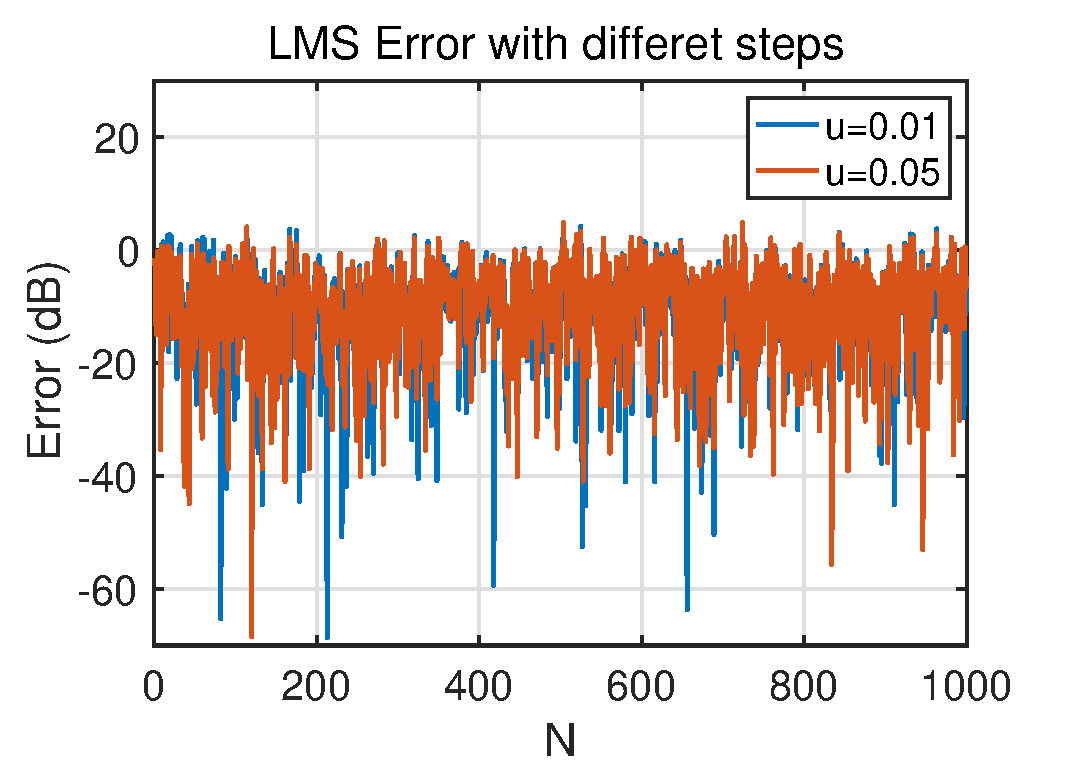
\includegraphics[width=\textwidth]{fig/21/21b1.eps}
     \end{subfigure}
     ~
     \begin{subfigure}[b]{0.4\textwidth}
         \centering
         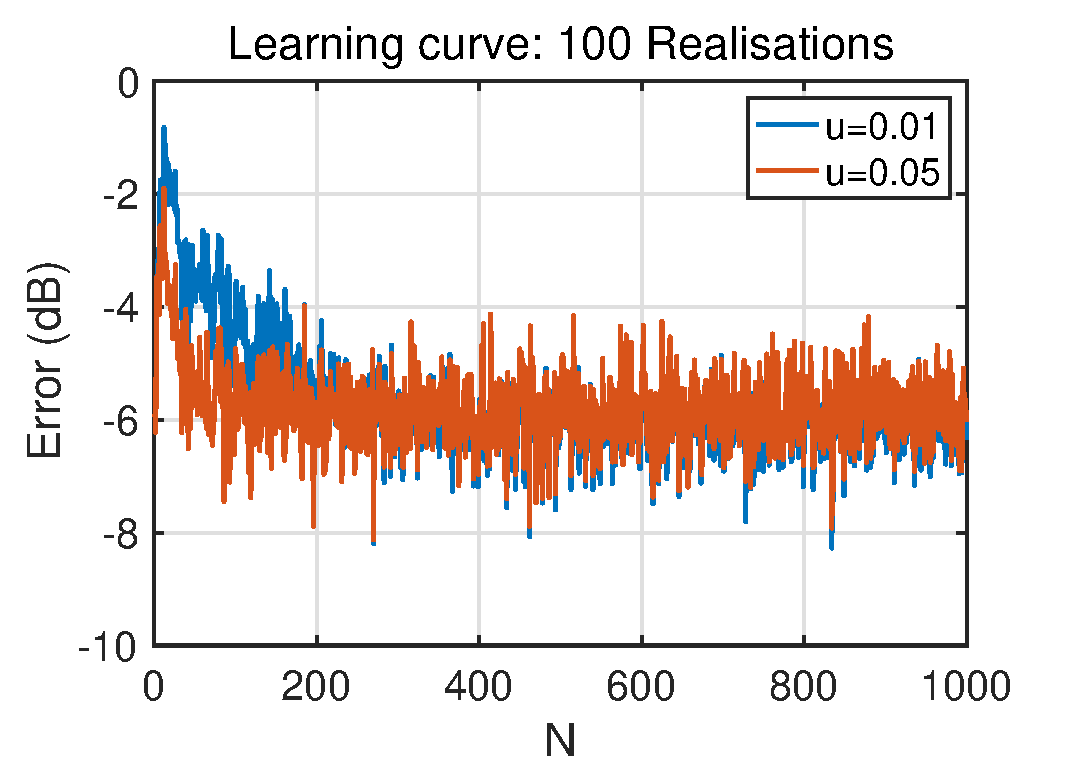
\includegraphics[width=\textwidth]{fig/21/21b2.eps}
     \end{subfigure}
        \caption{LMS estimated error with different realizations and steps}
        \label{fig:2_1_b}
\end{figure}
\subsection{Misadjustment of LMS}
The theoretical misadjustent of the LMS is approximated as $\mathcal{M}_{LMS} \approx \frac{\mu}{2}\mathrm{Tr}\{\mathbf{R}_{xx}\}$, where the autocorrelation matrix $\mathbf{R}_{xx}$ is calculated. However, the estimated misadjustment is the ratio of excess MSE and minimum MSE, which is $\mathcal{M}=\frac{MSE-\sigma^2}{\sigma^2}$. In addition, in order to guarantee the error calculated during steady state, the samples are selected after 400. Table.\ref{tab:M} shows the values of misadjustment. As shown in table, the measured MSE and misadjustment is slightly larger than theoretical values. However, small step size introduces a small misadjustment, whereas the convergence speed is slow..
\begin{table}[htp]
\centering
\caption{Theoretical and Actual Misadjustment values for step sizes}
\begin{tabular}{ |c|c|c| } 
 \hline
 $\mu$ & $\mathcal{M}_{LMS}$ & $\mathcal{M}$ \\ 
 \hline
 0.01 & 0.0093 & 0.0134
 \\ 
 \hline
 0.05 & 0.0463 & 0.0534
 \\ 
 \hline
\end{tabular}
\label{tab:M}
\end{table}
\subsection{LMS: estimated weights}
Fig.\ref{fig:2_1_d} depicts the estimated weights $a_1=0.1$ and $a_2=0.8$ with steps $\mu=0.01$ and $\mu=0.05$. Compared these estimated weights with true values, small step size provides an acceptable steady state error which is closer to actual weights. However, the convergence speed is relatively slow compared with large step size. On the contrast, when $\mu=0.05$, the convergence speed is significantly improved, resulting in a large difference with actual values. Thus, there is a trade-off between steady state error and convergence speed.
\begin{figure}[htp]
     \centering
     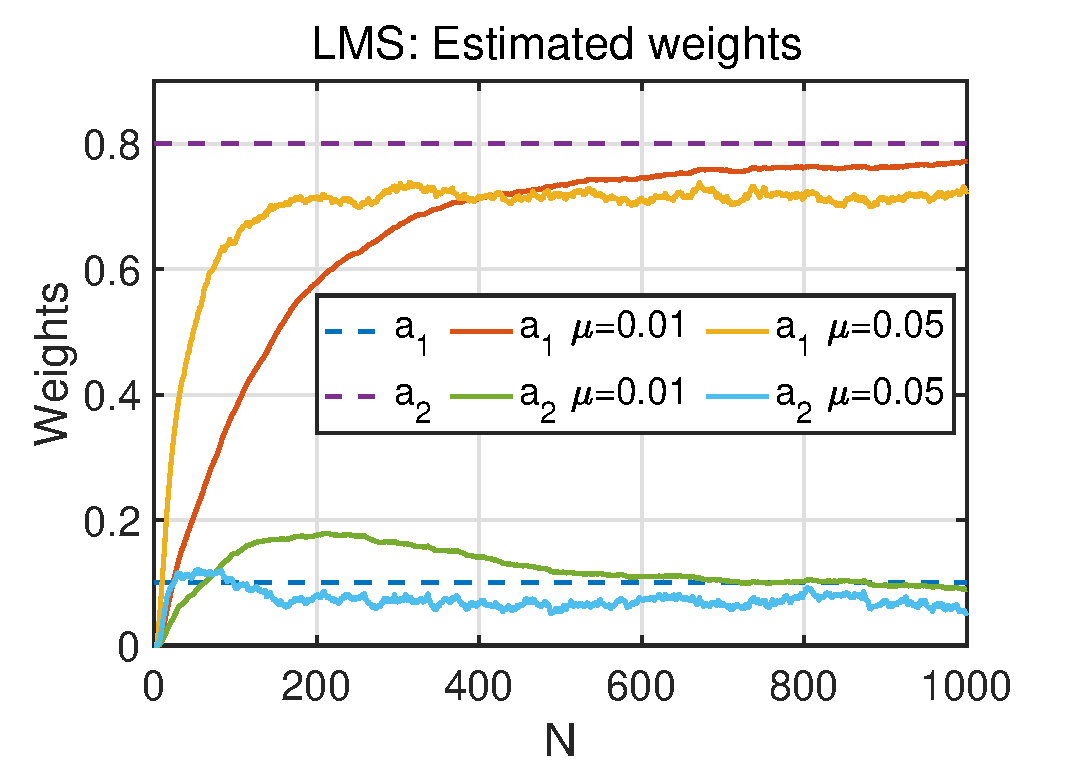
\includegraphics[width=0.4\textwidth]{fig/21/21d.eps}
     \caption{LMS estimated weights with different steps}
     \label{fig:2_1_d}
\end{figure}
\subsection{Leaky LMS}
For the leaky LMS, the cost function is 
\begin{align}
\mathcal J_2(n)&=\frac{1}{2}(e^2(n)+\gamma ||\mathbf {w}(n)||_2^2)\label{eq:cost2}\\
where \quad e(n)&=d(n)-\mathbf{w}_T(n)\mathbf {x}(n)\notag
\end{align}
To get the minimum squared error, the gradient with weight $\mathbf{w}$ of Eq.\ref{eq:cost2} is taken, 
\begin{align}
\nabla \mathcal J_2(n)&=\frac{1}{2}\partial (e^2(n)+\gamma ||\mathbf {w}(n)||_2^2)/\partial \mathbf {w}\notag\\
&=\frac{1}{2}(\frac{\partial(e^2(n))}{e(n)}\frac{\partial(e(n))}{\mathbf {w}}+2\gamma ||\mathbf {w}(n)||_2)\notag\\
&=-e(n)\mathbf{x}(n)+\gamma \mathbf {w}(n)
\label{eq:J2}
\end{align}
Therefore, the updated weight is 
\begin{align}
\mathbf {w}(n+1)&=\mathbf {w}(n)+\mu (-\nabla \mathcal J_2(n))\notag\\
				&=\mathbf {w}(n)+\mu (e(n)\mathbf{x}(n)-\gamma \mathbf {w}(n))\notag\\
				&=(1-\mu \gamma)\mathbf {w}(n)+\mu e(n)\mathbf{x}(n)
\label{eq:llms}
\end{align}
\subsection{Leaky LMS: estimated weights}
Fig.\ref{fig:2_1_f} illustrated the estimated weights using leaky LMS filter with $\gamma=$ 0.2, 0.4, 0.6 and $\mu=$ 0.01, 0.05. However, the estimated values converges to a certain value with a large difference with actual coefficient. With the incremental of $\gamma$, the steady state error significantly rises up. Observing weights curves, increasing $\gamma$ introduces a larger bias for lager weight than small weight. Thus, Leaky LMS causes large penalty for the large weight estimation.
\begin{figure}[htb]
     \centering
      \hspace{-0.4cm}
     \begin{subfigure}[b]{0.33\textwidth}
         \centering
         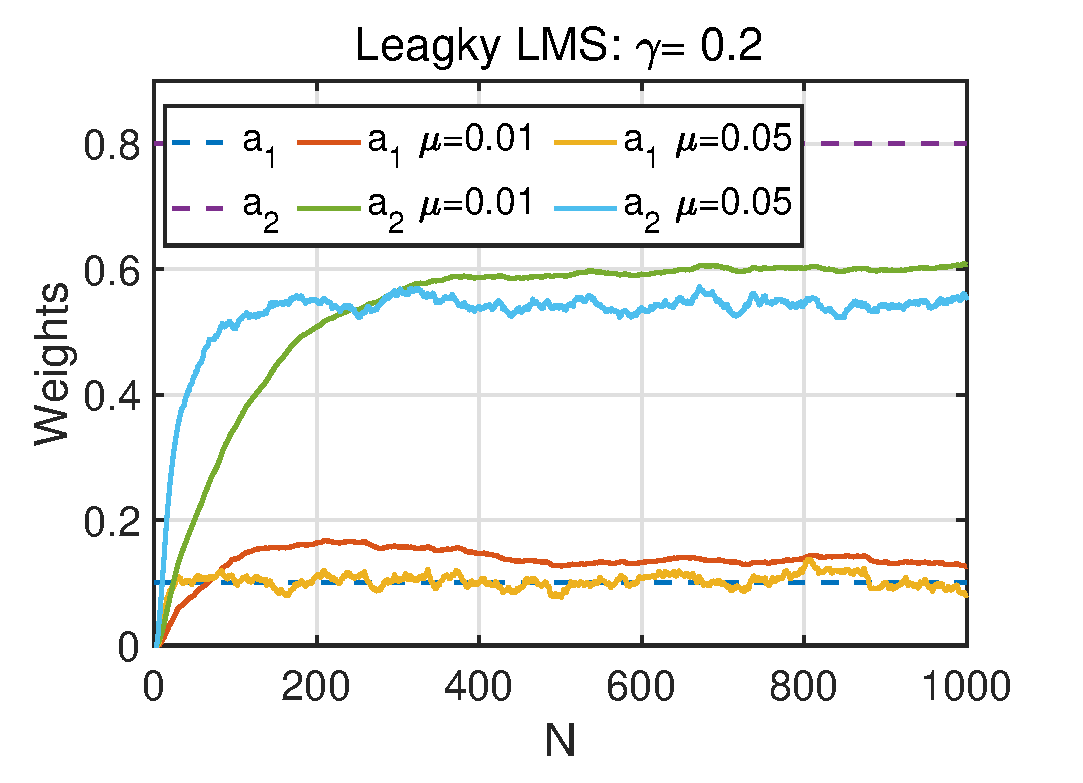
\includegraphics[width=\textwidth]{fig/21/21f1.eps}
     \end{subfigure}
     \hspace{-0.4cm}
     \begin{subfigure}[b]{0.33\textwidth}
         \centering
         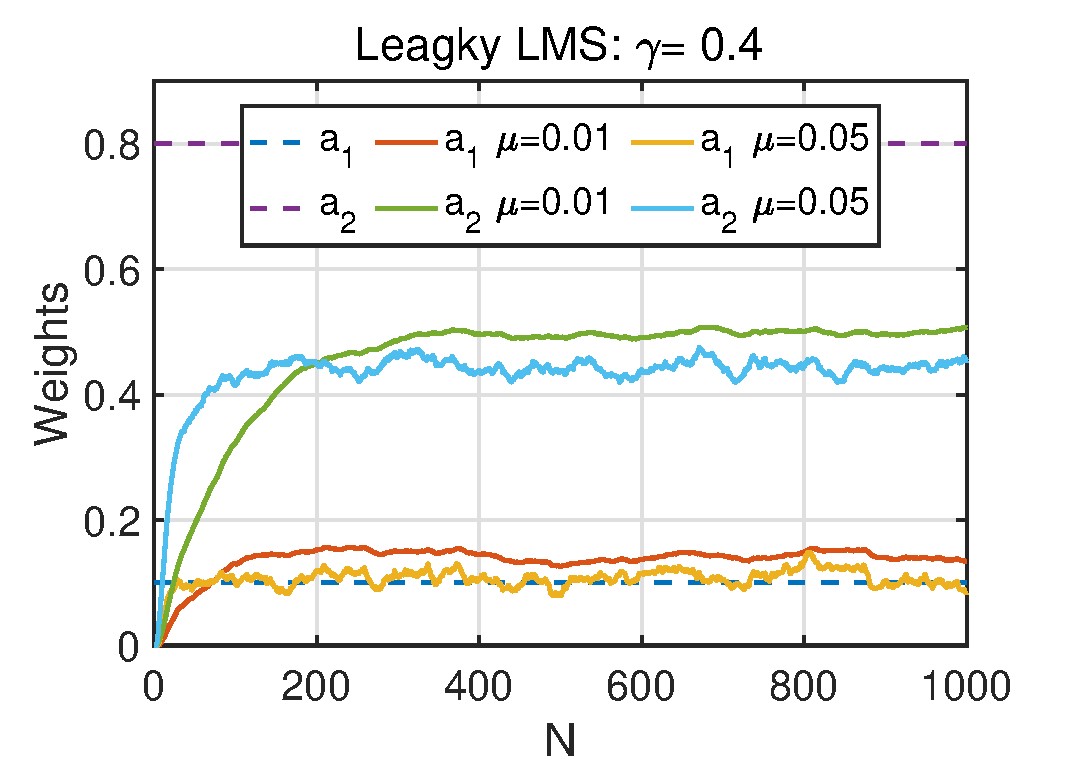
\includegraphics[width=\textwidth]{fig/21/21f2.eps}
     \end{subfigure}
      \hspace{-0.4cm}
     \begin{subfigure}[b]{0.33\textwidth}
         \centering
         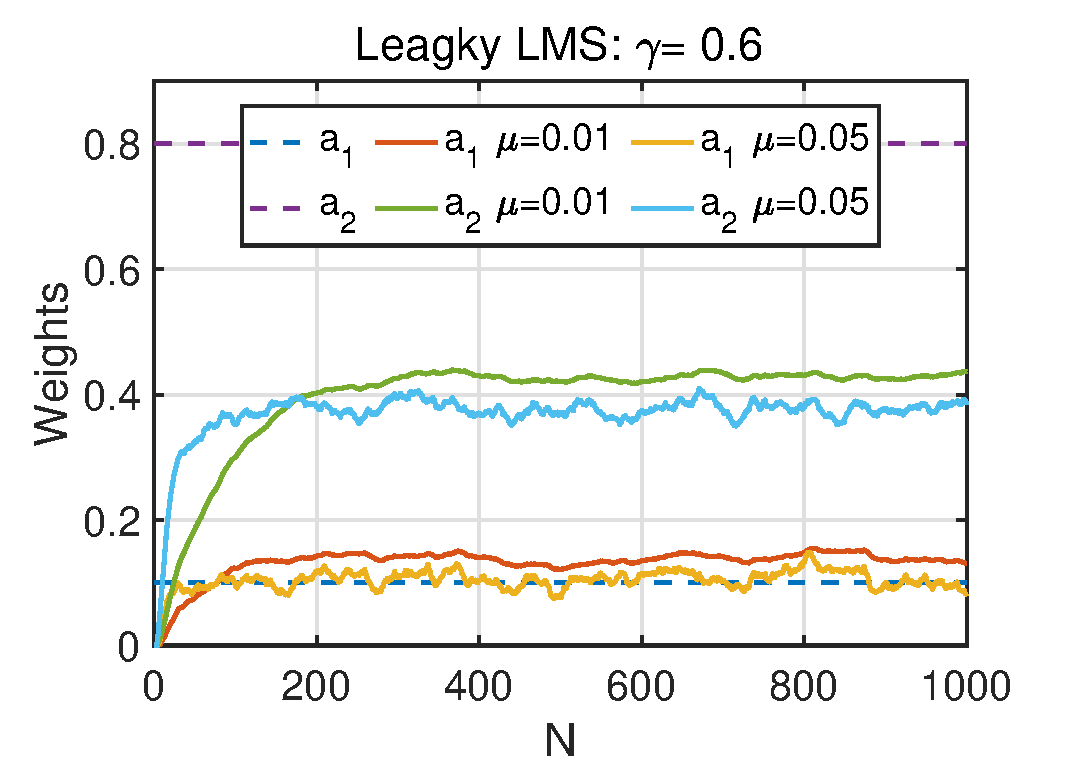
\includegraphics[width=\textwidth]{fig/21/21f3.eps}
     \end{subfigure}
        \caption{Leaky LMS estimated weights with different $\gamma$ and $\mu$}
        \label{fig:2_1_f}
\end{figure}\\
As to the general LMS algorithm, the optimal weight is
\begin{align}
 \mathbf {w}_{opt}=\mathbf{R}_{xx}^{-1} \mathbf{p}\quad \text{where} \quad \mathbf{p}= \mathbb{E}\{\mathbf{x}(n)d(n)\}
\end{align}
The autocorrelation matrix is semi-positive definite and can be invertible. However, the gradient vanishing problem is suffered when the eigenvalues of $\mathbf{R}_{xx}$ are zeros, resulting in divergence to expected values. By adding a small number $\gamma$ of $\mathbf{R}_{xx}$, the weights can converge, which is the purpose of Leaky LMS. Thus, the optimal weight is 
\begin{equation}
 \mathbf {w}_{opt}=(\mathbf{R}_{xx}+\gamma \mathbf{I})^{-1} \mathbf{p}
\end{equation}
Nevertheless, the eigenvalues of autocorrelation matrix are non-zeros for this experiment. Hence, adding large value of $\gamma$ leads to an obvious bias and the estimated weights converge to incorrect coefficients. 



